% tirlnx01 - Materiaal om het keuzevak Linux te geven 
% op de Hogeschool Rotterdam.
% Copyright (C) 2010 - 2011  Paul Sohier, Kevin van der Vlist
%
% This program is free software: you can redistribute it and/or modify
% it under the terms of the GNU General Public License as published by
% the Free Software Foundation, either version 3 of the License, or
% (at your option) any later version.
%
% This program is distributed in the hope that it will be useful,
% but WITHOUT ANY WARRANTY; without even the implied warranty of
% MERCHANTABILITY or FITNESS FOR A PARTICULAR PURPOSE.  See the
% GNU General Public License for more details.
%
% You should have received a copy of the GNU General Public License
% along with this program.  If not, see <http://www.gnu.org/licenses/>.
%
% Kevin van der Vlist - kevin@kevinvandervlist.nl
% Paul Sohier - paul@paulsohier.nl

\documentclass{beamer}

\mode<presentation>

\usepackage[dutch]{babel}
%\usepackage{beamerthemesplit}

\usepackage{listings}
%\usepackage{beamerthemesplit}

\lstset{ %
  language=bash,                % choose the language of the code
  basicstyle=\footnotesize,       % the size of the fonts that are used for the code
  numbers=left,                   % where to put the line-numbers
  numberstyle=\footnotesize,      % the size of the fonts that are used for the line-numbers
  numbersep=5pt,                  % how far the line-numbers are from the code
  showspaces=false,               % show spaces adding particular underscores
  showstringspaces=false,         % underline spaces within strings
  showtabs=false,                 % show tabs within strings adding particular underscores
  frame=lr,	                % adds left and right lines
  tabsize=2,	                % sets default tabsize to 2 spaces
  captionpos=b,                   % sets the caption-position to bottom
  breaklines=true,                % sets automatic line breaking
  breakatwhitespace=false,        % sets if automatic breaks should only happen at whitespace
%  escapeinside={\%*}{*)},         % if you want to add a comment within your code
  morekeywords={*,...}            % if you want to add more keywords to the set
}


\usetheme{Berlin}
\useinnertheme{rounded}
\usecolortheme{rose}
\setbeamertemplate{navigation symbols}{} 

\title{Keuzevak Linux - Week 5}
\author{Paul Sohier \and Kevin van der Vlist}
\institute{Versie $1.0$}
\date{\today}

\begin{document}

\begin{frame}
  \titlepage
\end{frame} 

\begin{frame}
  \frametitle{Inhoud}
  \tableofcontents
\end{frame}

%\section{Basiscommando's}
%\begin{frame}
%\frametitle{Basiscommando's}
%\begin{itemize}
%  \item 
%\end{itemize}
%\end{frame}

\section{Inleiding}

\begin{frame}
\frametitle{Shell - Inleiding}
\begin{figure}[H]
  \begin{center}
    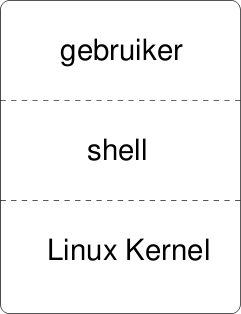
\includegraphics[scale=0.5]{images/shell_intro}
  \end{center}
  \caption{De basis}
  \label{fig:shell}
\end{figure}
\end{frame}

\begin{frame}
  \frametitle{Shell - Inleiding}
  \begin{itemize}
    \item<1-> \emph{Bourne Shell} (sh) orgineel
    \item<2-> \emph{Bourne Again Shell (Bash)} open source
    \item<3-> \emph{Debian Almquest Shell (Dash)} snellere afgeleide
    \item<4-> alles opgebouwd rondom Shell
  \end{itemize}
\end{frame}

\section{Theorie}
\begin{frame}
  \frametitle{Shell - Theorie}
  \begin{itemize}
    \item<1-> zie \texttt{man bash}
    \item<2-> \emph{any program that users employ to type commands}
    \item<3-> verschillende shells
    \item<4-> ook \emph{kde}, \emph{Gnome} zijn shells
  \end{itemize}
\end{frame}

\section{In/Output}
\begin{frame}
  \frametitle{Shell - In/Output}
  \begin{figure}[H]
    \begin{center}
      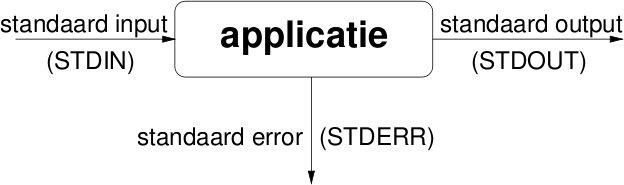
\includegraphics[scale=0.5]{images/inout}
    \end{center}
    \caption{In en Output}
    \label{fig:output}
  \end{figure}
\end{frame}

\begin{frame}[fragile]
  \frametitle{Shell - Pipeline}
  \begin{itemize}
    \item<1-> piping, doorsluizen van STDOUT naar een locatie, commando
    \item<2->
      \begin{lstlisting}
        grep kernel /var/log/syslog | more 
      \end{lstlisting}
    \item<3->
      \begin{lstlisting}
        grep bash /etc/passwd | sort > ~/bash_gebruikers.txt
      \end{lstlisting}
  \end{itemize}
\end{frame}

\begin{frame}[fragile]
  \frametitle{Shell - STDERR redirecten}
  \begin{itemize}
    \item<1-> STDERR naar file
      \begin{lstlisting}
        cat /etc/passwd | grep test 2> grep_errors.txt
      \end{lstlisting}
      \item<2-> STDOUT naar STDERROR
        \begin{lstlisting}
          cat /etc/passwd | grep test 1>&2
        \end{lstlisting}
      \item<3-> STDERR naar STDOUT
        \begin{lstlisting}
          cat /etc/passwrd | grep test 2>&1
        \end{lstlisting}
      \item<4-> STDERR en STDOUT naar 1 file/commando
        \begin{lstlisting}
          rm tmp/ -rfv &> /dev/null
        \end{lstlisting}
  \end{itemize}
\end{frame}

\section{Jobcontrol}
\begin{frame}[fragile]
  \frametitle{Shell - Jobcontrol}
  \begin{itemize}
    \item<1-> mutli tasking systeem
    \item<2-> opdracht draaien op achtergrond
      \begin{lstlisting}
        find / -name '*.txt*' > tekstbestanden &
        ls -IR / &
      \end{lstlisting}
      Dit geeft:
      \begin{lstlisting}
[1]- Running find / - name '*.txt *' > tekstbestanden &
[2]+ Running ls −lR / &        
      \end{lstlisting}
      Terughalen met \texttt{fg}
  \end{itemize}
\end{frame}

\end{document}
